\documentclass[conference]{IEEEtran}
\usepackage{cite}
\usepackage{amsmath,amssymb,amsfonts}
\usepackage{algorithmic}
\usepackage{graphicx}
\usepackage{textcomp}
\usepackage{xcolor}
\def\BibTeX{{\rm B\kern-.05em{\sc i\kern-.025em b}\kern-.08em
    T\kern-.1667em\lower.7ex\hbox{E}\kern-.125emX}}
\begin{document}

\title{Designing and Developing a Personalised Recommender System}

\author{\IEEEauthorblockN{lrfk99}
\IEEEauthorblockA{\textit{dept. Computer Science} \\
\textit{Durham University}\\
Durham, United Kingdom}
}

\maketitle


\section{Introduction}

\subsection{Domain of application}
The domain of this hybrid recommender system is restaurants, with a focus on trying new restaurants. 
This system is built around restaurants in a particular metropolitan area which serve a particular 
type of food. 

\subsection{Related work review}
Hybrid recommender systems which combine knowledge-based (KB) and collaborative-filtering (CF) techniques 
are designed to combine the ability of KB techniques to give generic recommendations to new users with 
small profiles and the strength of CF to find peer users with unexpected shared preferences. 
This combination of techniques is particularly well suited to restaurants since a user may often be in the 
mood for a specific type of food, such as Italian or Chinese, so they only want to see suggestions of that 
type or restaurant, which is where the knowledge-based recommender is helpful. 
A collaborative-filtering algorithm will then be able to order all the restaurants which match this 
explicit criteria by how the user should rate them, based on the opinions of other similar users, 
helping them to discover new restaurants to try. 
These techniques are used in the Entree restaurant recommender system \cite{burke1999integrating,burke2000knowledge,burke2002hybrid,burke2007hybrid}. 
In particular, Burke's 1999 paper \cite{burke1999integrating} is the first to discuss specifically using these 
two techniques in the same cascaded style that I implement here. 

\subsection{Purpose/Aim}
The purpose of this application is to give suitable suggestions of restaurants for a user to go to. 
The recommended restaurants should be in the metropolitan area which the user specifies, and serve the 
type of food that the user asks for. 
As well as fitting this explicit criteria, the suggested restaurants should be similar to other restaurants 
that the user has rated highly in the past and which other users with similar preferences also like. 
The system will allow the user to add ratings of the restaurants they are recommended, and these ratings will 
affect future suggestions the system gives for that user and other similar users. 


\section{Methods}

\subsection{Data description}
The data for my recommender system was generated from the Yelp Open Dataset \cite{YelpDataset}. 
This is a subset of all the businesses, reviews, and user data on Yelp, formatted as JSON files. 
The dataset includes approximately 8,000,000 reviews of 200,000 businesses by 2,000,000 users, as well as 
additional Covid-19 related features of each business such as whether they now offer takeout or delivery. 
There are 3 sections of the dataset, with 5 JSON files in the main dataset, 1 in the photos section, and 
1 in the covid section. 
The $business.json$ file contains business data including location data, attributes, and cuisine. 
$review.json$ contains full review text data including the $user\_id$ that wrote the review and the $business\_id$ 
that the review is written for. 
The file $user.json$ holds every user's first name along with other data adn metadata which I don't use \cite{YelpDataset}. 
The data files $checkin.json$ and $tip.json$ are not used in my system. 
The dataset also includes approximately 200,000 photos but these are not relevant to my application, since 
the interface is command line only, so they were discarded. 
The covid related data from $covid\_features.json$ contains additional information about each business with regards to 
the measures they have taken due to the pandemic, such as offering delivery or takeout options or a 
special message for customers. 
Every business in the dataset is in 1 of 10 metropolitan areas in the USA and Canada 
(Montreal, Calgary, Toronto, Pittsburgh, Charlotte, Urbana-Champaign, Phoenix, Las Vegas, Madison, and Cleveland) \cite{YelpDataset}. 

\subsection{Data preparation and feature selection}
The entire Yelp dataset contains a lot of data which is not relevant to my domain of restaurants, so much data 
preparation is required to save computation time and in order to provide more accurate predictions. 
The dataset is provided in JSON format, but in such a way that every entry is its own JSON on its own line, 
which does not lend well to fast lookups by the main program. 
Therefore it was necessary to convert every file I used in the system into a typical JSON file, such that it could 
be loaded as a python dictionary with the lookup key being either the uniquely identifying $business\_id$ or 
$user\_id$ depending on the case. 
This allows for extremely fast data lookups in the system. 
It was of course also necessary to filter the list of all Yelp businesses down to just the restaurants. 
I further narrowed the list of restaurants by selecting only those which fit into one or more of the top 12 
cuisines in terms of number of restaurants (American, Mexican, Italian, Chinese, Seafood, Japanese, Canadian, 
Mediterranean, Indian, Thai, Middle Eastern, Vietnamese, in that order). 
Since the user selects one of these 12 options for cuisines they want to find, they will 
never be recommended a restaurant which doesn't fit at least one of these categories. 
I chose to use the top 12 cuisines because it's enough to provide a wide variety of options to the user without 
being so many that the user is overwhelmed by the amount. 
I also ensured that every restaurant was still open and had at least 1 check-in in 2019 (the last year that 
data was available). 
This left 20,565 restaurants which could be recommended to the user, which needed to be split into their respective 
metropolitan areas by using the latitude and longitude values of the businesses and of the centres of each city. 
All other datasets were filtered to only data pertaining to these restaurants, with duplicates in the 
covid dataset removed. 
The reviews were further filtered to only those which had 5 or more 'useful' votes by other users. 
This was to ensure I was only using high quality reviews which others found helpful, as well as to allow the 
recommender system to compute results in a reasonable amount of time (~10 seconds on my machine). 
This left around 120,000 reviews, which were then converted to a CSV file ($reviews.csv$) with unnecessary data 
removed and structured as follows: ($User\_ID$, $Business\_ID$, $Rating$). 

\subsection{Hybrid scheme}
The two personalised recommender systems I implement are knowledge-based and collaborative-filtering, and 
the hybrid scheme is cascade. 
A cascade hybrid scheme works particularly well in my domain of restaurants with an emphasis on providing accurate 
predictions of restaurants which a user may like in a city they have never been to before, based on the restaurants 
they like in their home-city. 
This is because the knowledge-based system can filter the restaurants by location and by the type of food they serve, 
while the collaborative-filtering system is able to find restaurants which are similar to the ones the user has 
previously rated highly. 
So when these two systems are combined in a cascade style with the knowledge-based system as the primary recommender 
and the collaborative-filtering system as the secondary the hybrid system can find hidden similarities between 
restaurants in different cities very accurately. 
This method of hybrid recommender system (HRS) has been implemented as a restaurant recommender in the Entree 
system, giving very accurate results \cite{burke1999integrating,burke2000knowledge,burke2002hybrid,burke2007hybrid}. 

\subsection{Recommendation techniques/algorithms}
The first prediction method used in this hybrid system is a knowledge-based (KB) approach, which relies on knowledge 
about each of the restaurants based on its location and the type of food that it serves. 
This approach completely eliminates the cold-start problem, a new user will still receive relevant recommendations 
for the city they are in and the type of food they in the mood for when using a KB system. 
The second prediction method is a collaborative-filtering (CF) approach, specifically Single Value Decomposition (SVD) 
matrix factorisation. 
This approach was chosen because it scales well with large datasets, which is important since my dataset has 
~120,000 entries. 
The CF technique here also introduces an element of variability in the recommendations, such that the user 
may not receive the same ordering of suggestions when they run the system multiple times with the same 
KB specifications, helping the user to try new things. 
This system allows the user to make ratings through the user interface, providing the ability to experiment with 
the system in terms of how new ratings affect the current user's recommendations as well as those of other similar users. 

\subsection{Evaluation methods}
The evaluation of the system was done using offline experiments. 
The accuracy of ratings predictions was evaluated using Mean Absolute Error (MAE), which is calculated by the 
following equation:
\begin{equation}
    MAE = \frac{1}{|\mathcal{T}|} \sum_{(u,i)\in{\mathcal{T}}} {|\widehat{r}_{ui} - r_{ui}|}
\end{equation}
This metric is appropriate for this RS since it can handle large errors on a few items, which may occur in this system 
due to some rare skewed ratings. 
The MAE of this system is around 0.99. 

Measuring the accuracy of usage predictions is done using precision, calculated by: 
\begin{equation}
    Precision = \frac{TP}{TP+FP}
\end{equation}
where TP and FP correspond to True Positive and False Positive respectively. 
This is because the number of recommendations is predefined and not very large (8 items). 
The precision of this system is 0.125, since 1 out of the 8 items is a true positive. 

Coverage of the system is calculated by:
\begin{equation}
    Prediction\ coverage = \frac{|I_p|}{|I|}
\end{equation} 
where $I_p$ is the set of restaurants which can be recommended and $I$ is the set of all restaurants. 
In my system the coverage is ~0.32 ($\frac{20,565}{63,944}$), this is the most appropriate metric since 
the data for previously views items does not exist, ruling out novelty and diversity metrics. 

Explainability is measured holistically, by looking at the explanations given throughout the system and how 
well they describe the purpose of the recommendations, how accurately they match the mechanisms used to 
generate recommendations, how much they improve the system's transparency, and how they help users to make decisions 
more efficiently and effectively. 
Generally the explainability of this system is quite high with regards to all four of these criteria. 

\section{Implementation}

\subsection{Input interface}
The system has a command line based interface, so all user input of the input is given via the command line. 
The system recognises the active user by their unique user ID, some example IDs are provided in the 'README.txt' 
file for testing and demonstration purposes. 
Only explicit user data is gathered in order to make the system more explainable and transparent, 
and users are made aware of which data is collected, how it is collected, and for which purposes. 
This data includes the user's nearest city (of the 10 available) and the type of food that 
they are in the mood for. 
The user is able to change these choices from the main menu, as well as switch to a different user 
for testing purposes. 
When the user is presented with a list of recommendations, they can then choose one that they want 
to see more information about and from here they can leave a rating, return to the list, or return to 
the main menu. 
User profiles can be updated by giving a rating of a restaurant through the system. 
Any rating given will affect future recommendations given by the system to that user 
and to other similar users. 

\subsection{Recommendation algorithm}
The collaborative-filtering aspect of the algorithm is carried out by first converting the ratings data to a 
matrix with $User\_ID$ as the rows and $Business\_ID$ as the columns. 
If a user has not rated a restaurant then the rating in that cell is set to 0. 
The prediction $\widehat{r}_{ui}$ (user $u$'s rating of item $i$) is set as:
\begin{equation}
    \widehat{r}_{ui} = \mu + b_u + b_i + q_i^Tp_u
\end{equation}
Where the parameters are learnt by minimising the following regularised squared error: 
\begin{equation}
    \sum_{r_{ui}\in{R_{train}}} (r_{ui} - \widehat{r}_{ui})^2 + \lambda(b_i^2 + b_u^2 + ||q_i||^2 + ||p_u||^2)
\end{equation}
This minimisation is performed by stochastic gradient descent:
\begin{align}
    \begin{split}
    & b_u \gets b_u + \gamma(e_{ui} - \lambda b_u) \\
    & b_i \gets b_i + \gamma(e_{ui} - \lambda b_i) \\ 
    & p_u \gets p_u + \gamma(e_{ui} \cdot q_i - \lambda p_u) \\ 
    & q_i \gets q_i + \gamma(e_{ui} \cdot p_u - \lambda q_i) \\
    \end{split}
\end{align}
where $e_{ui} = r_{ui} - \widehat{r}_{ui}$. 
These steps are performed over all the ratings of the trainset and repeated 20 times \cite{SVD}. 
The knowledge-based aspect of the algorithm produces recommendations based on the explicit location and cuisine 
preferences of the user. 
These are then cascaded down to the CF algorithm, which assigns each a predicted rating based on the ratings data. 
The 8 recommendations with the highest predicted rating are then presented to the user. 

\subsection{Output interface}
Recommendations and prediction scores are presented to the user via the command line interface and using an ASCII table. 
I used a python module called texttable for this, since it makes the output very clear and visually appealing. 
I chose to output the top 8 recommendations since I think this is enough variety and choice for the user to find 
a restaurant to try, without there being too many options which might overwhelm the user. 
If I presented more than 8 recommendations at a time, the table wouldn't fit in a single terminal output window and 
would require the user to scroll around to read different parts of the output. 
Since the user will be interacting with the system on a laptop or desktop computer through a command line interface, 
an ASCII table is the most visually attractive way to present information, and the white text on a (typically) black 
background will help accommodate users who are colourblind or who require a high-contrast interface. 
The interface is clear enough to understand that users of all ages are able to use the system, and if a user 
requires the text to be larger then they can increase the text size of their terminal. 
Along with the recommended restaurants, an explanation of how these results are calculated is also provided, as 
well as the prediction values themselves so the user can understand why they are being shown these suggestions. 
This, along with an option in the main menu to view information about the data the system uses and how it is used, 
further adds to the explainability and transparency. 
\begin{figure}
    \centering
    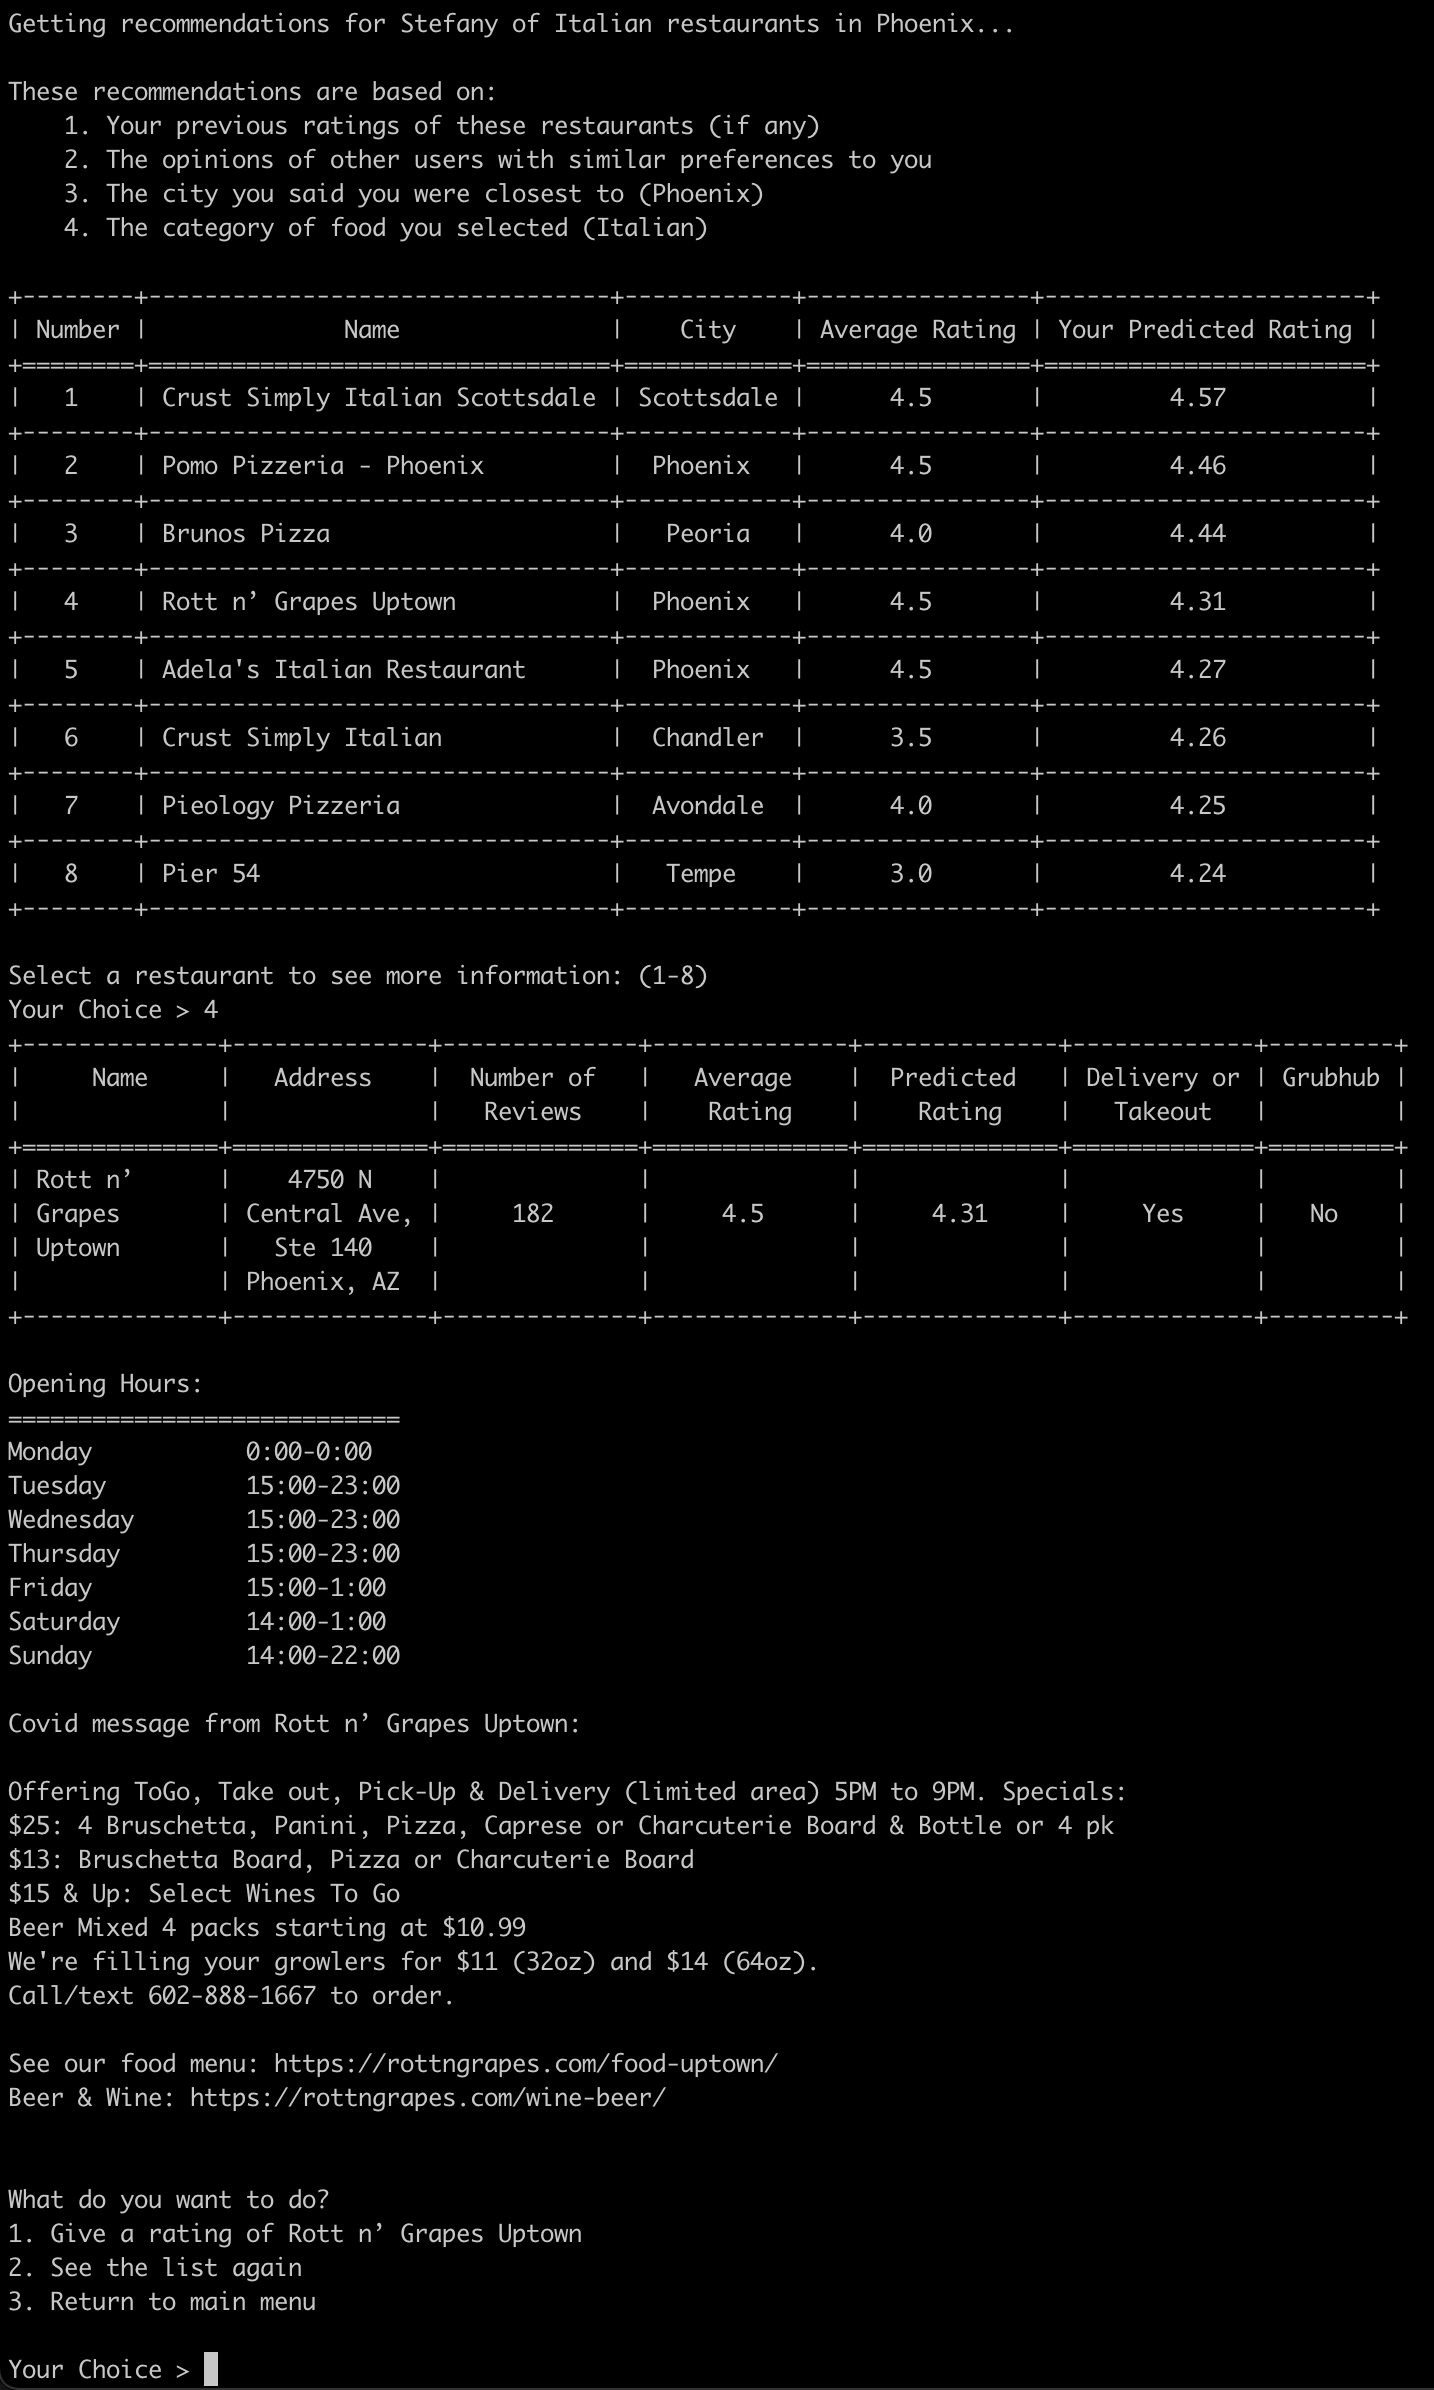
\includegraphics[width=0.4\linewidth]{output.png}
    \caption{System output}
    \label{fig:output}
\end{figure}


\section{Evaluation results}

\subsection{Comparison against baseline implementation}
Cross validation with 5 folds was carried out on both the SVD system and a baseline implementation. 
The 5 Mean Absolute Errors for the SVD system had a mean of 0.9962 and a standard deviation of 0.0033. 
The MAE results for the baseline implementation had a mean of 1.0091 and a standard deviation of 0.0056. 
This shows that when compared to a baseline implementation, the SVD system does perform better, generating more 
accurate predictions, however the difference is not particularly large. 

\subsection{Comparison against hybrid recommenders in related studies}
The Entree restaurant recommender system is an example of a cascade style hybrid recommender system which 
uses both knowledge-based and collaborative-filtering methods to help users find a restaurant they might like in 
a city they've never been to before \cite{burke1999integrating,burke2000knowledge,burke2002hybrid,burke2007hybrid}. 
This is very similar to the way my system works, with the biggest difference being the vastly greater amount of 
knowledge engineering that has gone into Entree. 
This additional knowledge is used in Entree, and other FindMe style systems, to give more accurate similarity assessments 
of restaurants by considering factors such as price and quality of experience as well as location and cuisine, 
and by arranging these factors hierarchically. 
For example, Entree arranges these as: cuisine, price, quality of experience, others, but other systems allow the 
user to specify this order themselves. 
This is part of the reason why Entree would outperform this system. 

\subsection{Ethical issues}
One ethical issue resulting from data collection is whether people who use Yelp are aware that some of their 
personal data is being made publicly available as part of a large dataset. 
An approach to solve this issue would be an opt-in for whether a user wants to allow their data to be used in this way. 
Another issue is a business which has received unfair negative reviews, my recommender system would be less likely to 
suggest this restaurant to a user, causing the owner to unfairly lose business. 
This can be solved by moderation of reviews and allowing business owners to appeal negative reviews. 
A third issue arising from this system is that users now don't need to visit the Yelp website to find restaurant 
recommendations, meaning that Yelp will lose ad-revenue due to reduced site-traffic. 
Yelp could address this issue by introducing additional useful features to their website which are not available in 
this system, such that users would want to visit Yelp.com for their recommendations. 


\section{Conclusion}

\subsection{Limitations}
Currently the system cannot consider the user's preferences in terms of pricing of a restaurant, and it also does 
not have precise location information, only the metropolitan area the user is in or near to. 
This means that how central a restaurant is to the city centre currently has no impact on the recommendations. 

\subsection{Further developments}
The system could be developed further by implementing the idea of particular cuisines being more similar 
to some than others. 
The user could also specify an acceptable price range that they are looking for, and the system could make 
recommendations based on estimated or known demographic information of the user. 


\bibliographystyle{IEEEtran}
\bibliography{IEEEabrv,references}


\end{document}
